\documentclass[CJKutf8,xcolor=pdftex,dvipsnames,table]{beamer}
\usepackage{hyperref}
\hypersetup{
  pdftitle={Operating System Concepts},
  pdfauthor={Hong MingJian},
  pdfsubject={File System},
  pdfpagemode={FullScreen},
  colorlinks={true},
  linkcolor={blue},
}
\usepackage{CJKutf8}

\usetheme{Madrid}%{Warsaw}
\usecolortheme{crane}

%gets rid of bottom navigation bars
\setbeamertemplate{footline}[page number]{}
%gets rid of navigation symbols
\setbeamertemplate{navigation symbols}{}

\begin{document}
\begin{CJK*}{UTF8}{song}

  \title{\CJKfamily{hei} 操作系统原理}
  \subtitle{\CJKfamily{hei} 第十一章:文件系统}
  \author{\CJKfamily{hei} 洪明坚}
  \institute{\CJKfamily{hei} 重庆大学软件学院}
  \date{\today}
  
  \AtBeginSection[]
  {
    \begin{frame}
      \frametitle{Outline}
      \tableofcontents[currentsection]
    \end{frame}
  } 
  
  \frame{\titlepage}

  \frame{\frametitle{目录}\tableofcontents}

  \section{File system interface}
  
  \subsection{File concept}
  
  %% PAGE
  \begin{frame}
    \frametitle{File concept} \pause
    \begin{itemize}
    \item Logical contiguous secondary storage \pause
      \begin{itemize}
      \item The smallest allotment of logical continuous secondary storage from a user's perspective \pause
      \end{itemize}
    \item Types \pause
      \begin{itemize}
      \item Data \pause
        \begin{itemize}
        \item numeric \pause
        \item character \pause
        \item binary \pause
        \item ...... \pause
        \end{itemize}
      \item Program
      \end{itemize}
    \end{itemize}
  \end{frame}

  %% PAGE
  \begin{frame}
    \frametitle{File structure (1/2)} \pause
    \begin{itemize}\parskip=0pt
    \item None - just a sequence of bytes \pause
    \item Simple record structure \pause
      \begin{itemize}\parskip=0pt
      \item Lines \pause
      \item Fixed length \pause
      \item Variable length \pause
      \end{itemize}
    \item Complex structures
      \begin{itemize}\parskip=0pt
      \item Formatted document \pause
      \item Object file \pause
      \item Executable file \pause
      \end{itemize}
    \item Who decides? \pause
      \begin{itemize}\parskip=0pt
      \item Operating system \pause
        \begin{itemize}\parskip=0pt
        \item Structure of the executable file and shared library file \pause
        \end{itemize}
      \item Program
      \end{itemize}
    \end{itemize}
  \end{frame}

  %% PAGE
  \begin{frame}
    \frametitle{File structure (2/2)} \pause
    \begin{center}
      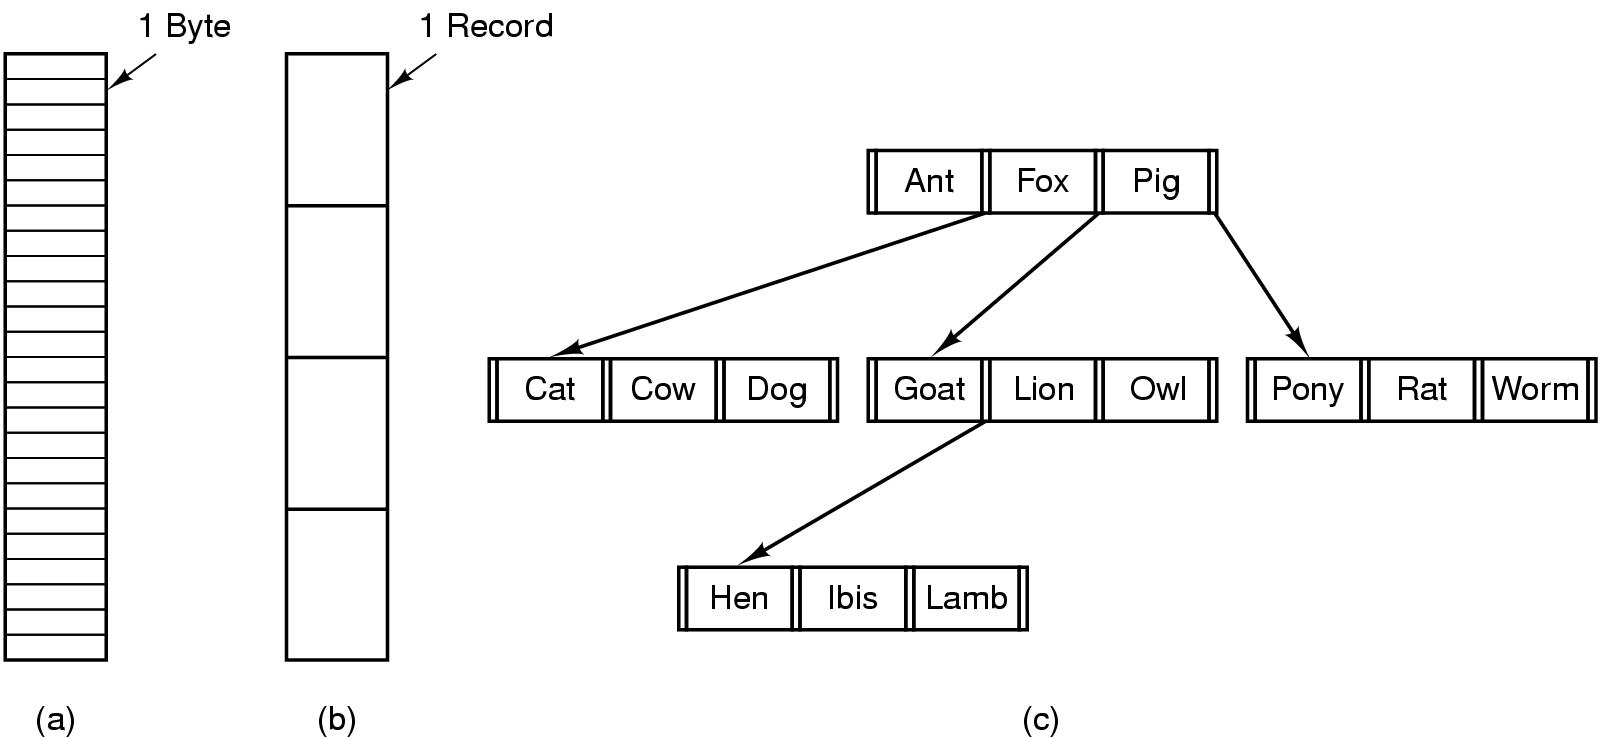
\includegraphics[scale=0.2]{mosv2f6-2}
    \end{center}
  \end{frame}

  %% PAGE
  \begin{frame}
    \frametitle{File attributes} \pause
    \begin{itemize}
    \item Name \pause - only information kept in human-readable form \pause
    \item Type \pause - needed for systems that support different types \pause
    \item Location \pause - pointer to data blocks on the device \pause
    \item Size \pause - current file size \pause
    \item Protection \pause - controls who can do reading, writing and executing \pause
    \item Time, date and user identification \pause - data for protection, security and usage monitoring \pause
    \item All these information about files are kept in the directory structure, which is maintained on the device
    \end{itemize}
  \end{frame}

  %% PAGE
  \begin{frame}
    \frametitle{File operations} \pause
    \begin{itemize}
    \item Create, Open, Close, Read, Write, Seek, Delete \pause
    \item Open files \pause
      \begin{itemize}
      \item When a file has been opened, in addition to the information stored on the device, several pieces of data are needed to manage open files \pause
        \begin{itemize}
        \item File pointer \pause - pointer to last read/write location, per process that has the file open \pause
        \item File-open count \pause - counter of number of times a file is open to allow removal of data from open-file table when the last process closes it \pause
        \item Device location of the file \pause - cache of data access information \pause
        \item Access rights \pause - per-process access mode information
        \end{itemize}
      \end{itemize}
    \end{itemize}
  \end{frame}

  %% PAGE
  \begin{frame}
    \frametitle{File types} \pause
    \begin{itemize}
    \item The content of a file determines its type. \pause
    \item How does the user know the type of a file? \pause
      \begin{itemize}
      \item Include the type as part of the file name called the \emph{extension}.\pause
      \end{itemize}
    \end{itemize}
    \begin{center}
      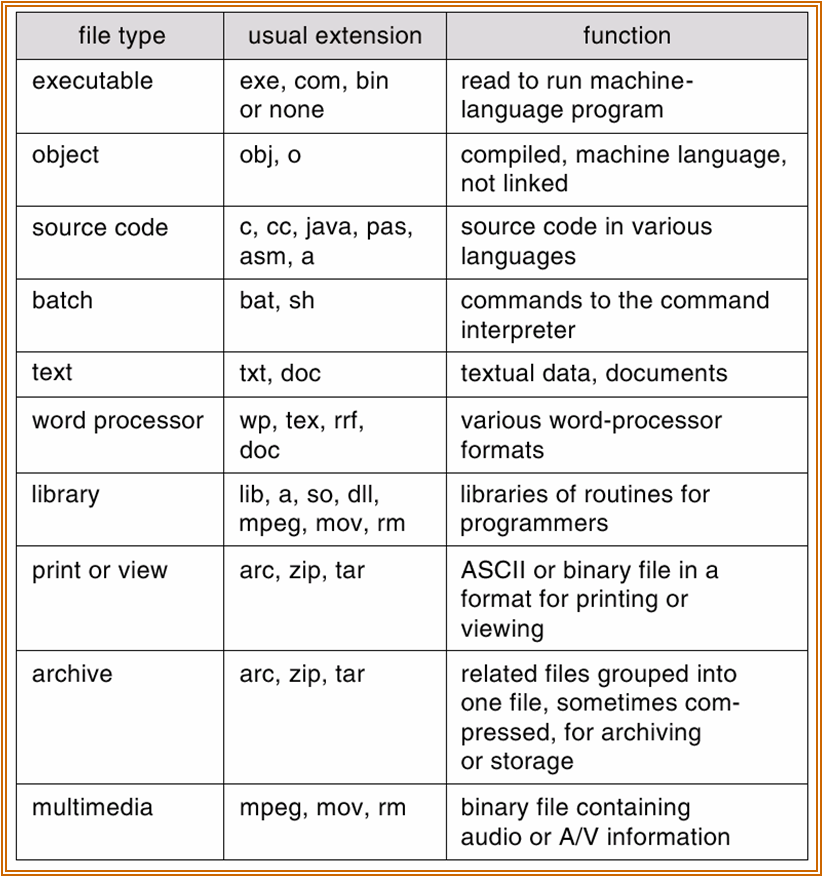
\includegraphics[scale=0.4]{v6f11-1}
    \end{center}
  \end{frame}

  \subsection{Access methods}

  %% PAGE
  \begin{frame}
    \frametitle{File access} \pause
    \begin{itemize}
    \item Sequential access \pause
      \begin{itemize}
      \item read all bytes/records from the beginning \pause
      \item cannot jump around, but could rewind or back up \pause
      \item convenient when the device is magnetic tape\pause
      \end{itemize}
    \item Random access \pause
      \begin{itemize}
      \item bytes/records read in any order \pause
      \item essential for database systems
      \end{itemize}
    \end{itemize}
  \end{frame}

  %% PAGE
  \begin{frame}
    \frametitle{Questions}
    \begin{itemize}
    \item Any questions?
    \end{itemize}
    \begin{center}
      
\includegraphics[scale=.5]{question}
    \end{center}
  \end{frame}

  \subsection{Directory structure}

  %% PAGE
  \begin{frame}
    \frametitle{Directory structure} \pause
    \begin{itemize}
    \item File system resides on the devices, such as disk and tape. \pause
      \begin{itemize}
      \item Usually, devices are split into one or more \emph{partitions} on which the file systems reside. \pause
      \end{itemize}
    \item To better organize files within a file system, \emph{directory} is used to group files. \pause
    \end{itemize}
    \begin{center}
      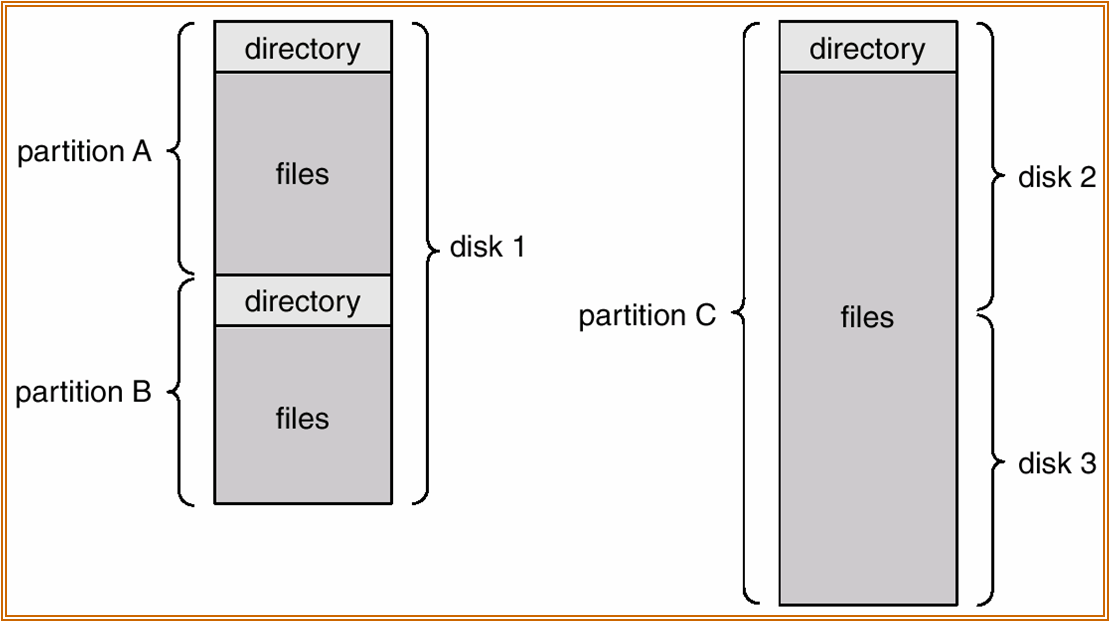
\includegraphics[scale=.4]{v6f11-5}
    \end{center}
  \end{frame}

  %% PAGE
  \begin{frame}
    \frametitle{Directory operations} \pause
    \begin{itemize}
    \item Search for a file \pause
    \item Create a file \pause
    \item Delete a file \pause
    \item List a directory \pause
    \item Rename a file \pause
    \item Traverse the entire file system
    \end{itemize}
  \end{frame}

  %% PAGE
  \begin{frame}
    \frametitle{Single-level directory} \pause
    \begin{center}
      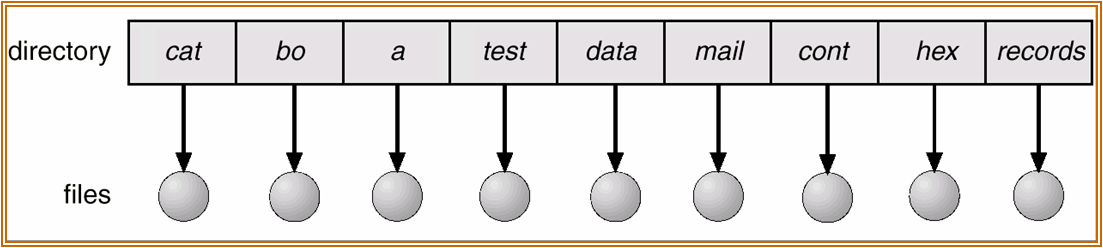
\includegraphics[scale=.5]{v6f11-6} \pause
    \end{center}
    \begin{itemize}
    \item Limitations \pause
      \begin{itemize}
      \item Naming problem \pause
      \item Grouping problem
      \end{itemize}
    \end{itemize}
  \end{frame}

  %% PAGE
  \begin{frame}
    \frametitle{Two-level directory} \pause
    \begin{itemize}
    \item Separate directory for each user \pause
    \end{itemize}
    \begin{center}
      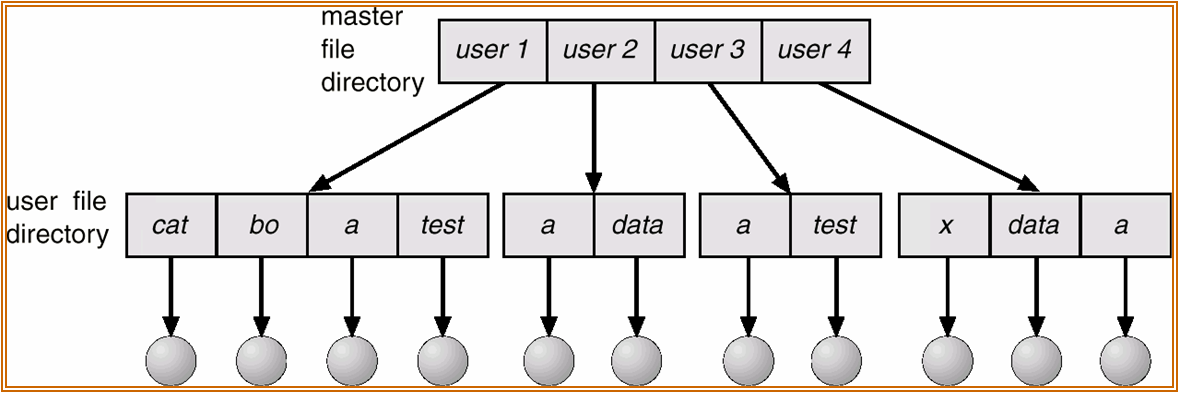
\includegraphics[scale=.5]{v6f11-7} \pause
    \end{center}
    \begin{itemize}
    \item Features \pause
      \begin{itemize}
      \item Files or directories can be located by its \emph{path} \pause
      \item Can have the same file name for different users
      \end{itemize}
    \end{itemize}
  \end{frame}

  %% PAGE
  \begin{frame}
    \frametitle{Tree-structured directory} \pause
    \begin{center}
      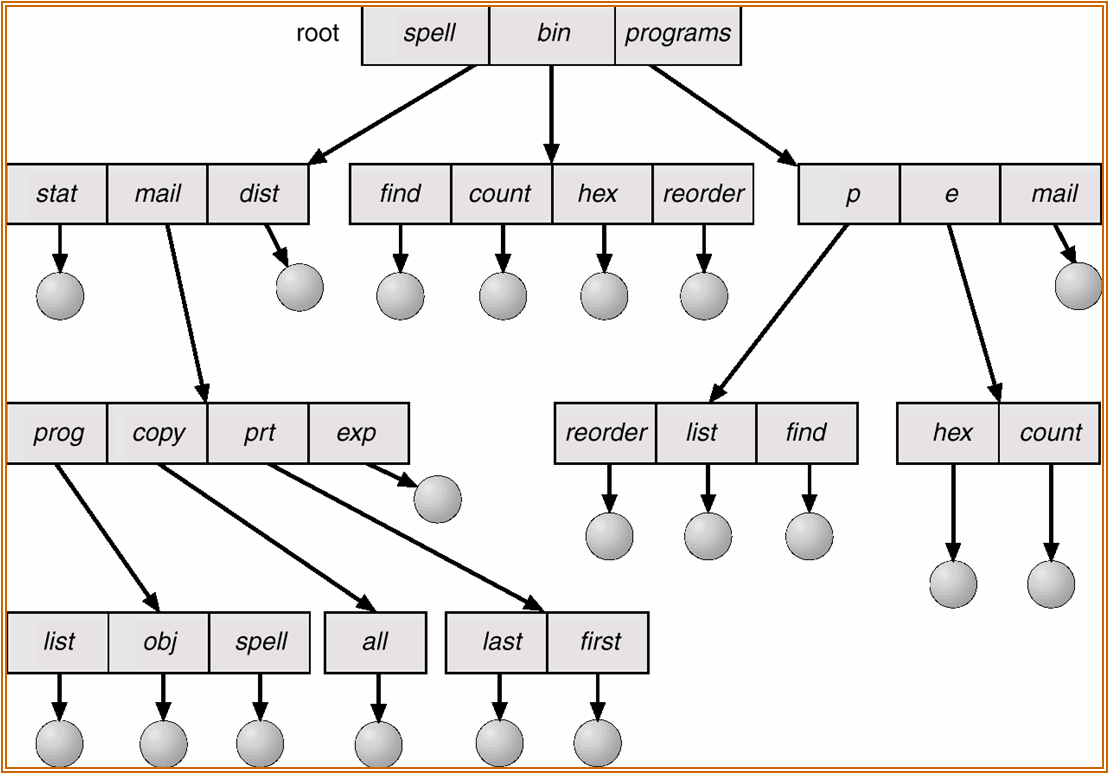
\includegraphics[scale=.4]{v6f11-8} \pause
    \end{center}
    \begin{itemize}\parskip=0pt
    \item Features \pause
      \begin{itemize}\parskip=0pt
      \item Grouping capability \pause
      \item \emph{Absolute} or \emph{relative} path \pause
      \item \emph{Working} (\emph{current}) directory of each process
      \end{itemize}
    \end{itemize}
  \end{frame}

  %% PAGE
  \begin{frame}
    \frametitle{Acyclic-graph directory} \pause
    \begin{center}
      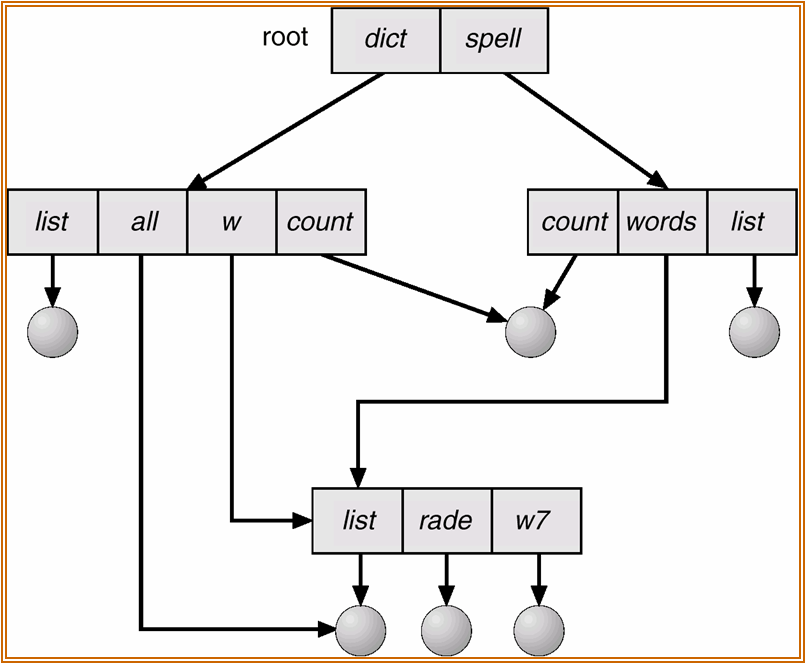
\includegraphics[scale=.4]{v6f11-9} \pause
    \end{center}
    \begin{itemize}
    \item Features \pause
      \begin{itemize}
      \item Two different names of the same file, i.e., \emph{aliasing} \pause
      \item Dangling pointer problem \pause
        \begin{itemize}
        \item Some operating systems do not support acyclic-graph directory, such as MS-DOS \pause
        \item UNIX/LINUX and Windows (7+) support it via \htmladdnormallink{\emph{symbol link}}{https://en.wikipedia.org/wiki/Symbolic\_link}
        \end{itemize}
      \end{itemize}
    \end{itemize}
  \end{frame}

  %% PAGE
  \begin{frame}
    \frametitle{Questions}
    \begin{itemize}
    \item Any questions?
    \end{itemize}
    \begin{center}
      
\includegraphics[scale=.5]{question}
    \end{center}
  \end{frame}

  \subsection{File system mounting}

  %% PAGE
  \begin{frame}
    \frametitle{File system mounting (1/2)} \pause
    \begin{itemize}
    \item A file system which resides on the device must be \emph{mounted} to be accessed. \pause
      \begin{itemize}
      \item The place where the file system is mounted is named \emph{mount point}.\pause
      \item Typically, a mount point is an empty directory. \pause
      \end{itemize}
    \item For example, Windows operating systems mount any partitions which contain the FAT(-12, -16, -32) or NTFS file system at ``C:'', ``D:'' and so on during the booting process. \pause
    \item While in the UNIX/Linux, system administrators must issue a command to mount a file system within a device. \pause
      \begin{itemize}
      \item \emph{mount -t iso9660 /mnt/cdrom /dev/cdrom}
      \end{itemize}
    \end{itemize}
  \end{frame}

  %% PAGE
  \begin{frame}
    \frametitle{File system mounting (2/2)} \pause
    \begin{center}
      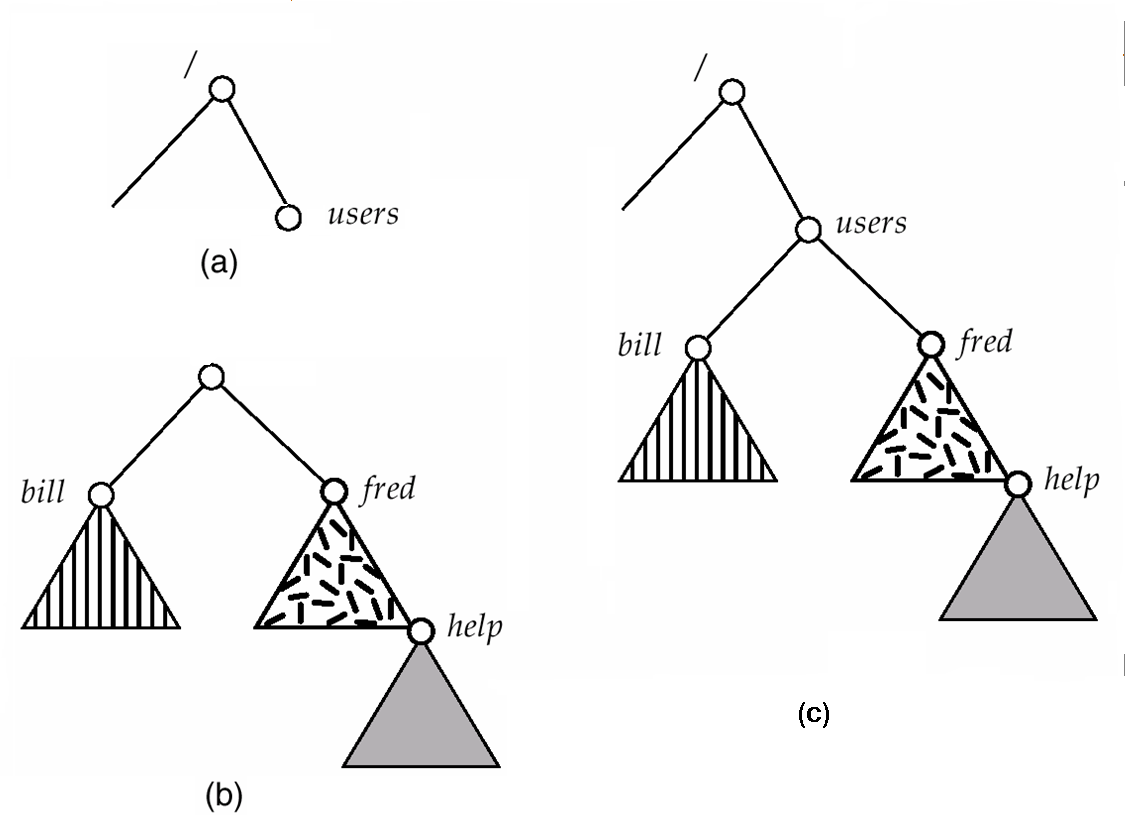
\includegraphics[scale=.15]{v6f11-11x} \pause
    \end{center}
    \begin{itemize}\parskip=0pt
    \item Example \pause
      \begin{itemize}\parskip=0pt
      \item An existing mounted file system, figure (a) \pause
      \item An unmounted file system resides on a disk, figure (b) \pause
      \item After mounting the file system (b) on the directory of existing file system ``/users'', figure (c)
      \end{itemize}
    \end{itemize}
  \end{frame}

  %% PAGE
  \begin{frame}
    \frametitle{Questions}
    \begin{itemize}
    \item Any questions?
    \end{itemize}
    \begin{center}
      
\includegraphics[scale=.5]{question}
    \end{center}
  \end{frame}

  \subsection{File sharing}

  %% PAGE
  \begin{frame}
    \frametitle{File sharing} \pause
    \begin{itemize}
    \item Sharing of files on multi-user systems is desirable. \pause
      \begin{itemize}
      \item Most systems identify the users by its unique \emph{user identification}, or \emph{UID} \pause
      \item In addition to UID, some systems also implement the \emph{group} functionality \pause
        \begin{itemize}
        \item Each group is assigned an unique \emph{group identification}, or \emph{GID} \pause
        \end{itemize}
      \item Every users can be in one or more groups \pause
      \end{itemize}
    \item When a file or directory is initially created, it is associated with the UID and GID of the user. \pause
      \begin{itemize}
      \item The user who owns a file is the \emph{owner} of the file.
      \end{itemize}
    \end{itemize}
  \end{frame}

  \subsection{Protection}

  %% PAGE
  \begin{frame}
    \frametitle{Protection} \pause
    \begin{itemize}\parskip=0pt
    \item File owner should be able to control \pause
      \begin{itemize}\parskip=0pt
      \item What can be done and \pause
      \item by whom \pause
      \end{itemize}
    \item Types of access \pause
      \begin{itemize}\parskip=0pt
      \item Read (R), Write (W), Execute (X), Append, Delete, List
      \end{itemize}
    \end{itemize}
  \end{frame}

  %% PAGE
  \begin{frame}
    \frametitle{UNIX/Linux file and directory protection} \pause
    \begin{itemize}
    \item Three classes of users and their access rights
      \begin{itemize}\parskip=0pt
      \item \color{red}owner\color{black} \  with  her/his  RWX \pause
      \item \color{blue}group\color{black} \  with  their    RWX \pause
      \item \color{green}public\color{black} \  with  their    RWX \pause
      \end{itemize}
    \item Example \pause
      \begin{itemize}
      \item \emph{-\color{red}rw-\color{blue}rw-\color{green}r---\color{black} \  1 \color{red}hmj\color{black} \color{blue}devel\color{black} 525 2007-04-27 23:52 vmmap.c}
      \end{itemize}
    \end{itemize}
  \end{frame}

  %% PAGE
  \begin{frame}
    \frametitle{Access-control list} \pause
    \begin{itemize}
    \item The \emph{access-control list (ACL)} specifies the user name and the types of access allowed for each user. \pause
      \begin{itemize}
      \item It's used to enforce fine-grained file and directory protection. \pause
      \end{itemize}
    \item The main problem with ACL is their length. \pause
      \begin{itemize}
      \item So, the most common approach is to combine the UNIX-style protection with the ACL. \pause
      \item For example, Windows NT or later and Solaris 2.6 or later use this combined approach.
      \end{itemize}
    \end{itemize}
  \end{frame}
  
  %% PAGE
  \begin{frame}
    \frametitle{Questions}
    \begin{itemize}
    \item Any questions?
    \end{itemize}
    \begin{center}
      
\includegraphics[scale=.5]{question}
    \end{center}
  \end{frame}
  
  \section{File system implementation}

  \subsection{File system structure}

  %% PAGE
  \begin{frame}
    \frametitle{File system structure} \pause
    \begin{itemize}\parskip=0pt
    \item File \pause
      \begin{itemize}\parskip=0pt
      \item Logical storage unit \pause
      \item Collection of related information \pause
      \item \emph{File Control Block (FCB)} contains all meta-information of a file \pause
        \begin{itemize}\parskip=0pt
        \item In UNIX, FCB is usually called \emph{inode} \pause
        \end{itemize}
      \end{itemize}
    \item A file system resides on the secondary storages and is organized into layers
    \end{itemize}
  \end{frame}

\iffalse
  %% PAGE
  \begin{frame}
    \frametitle{Layered File system} \pause
    \begin{center}
      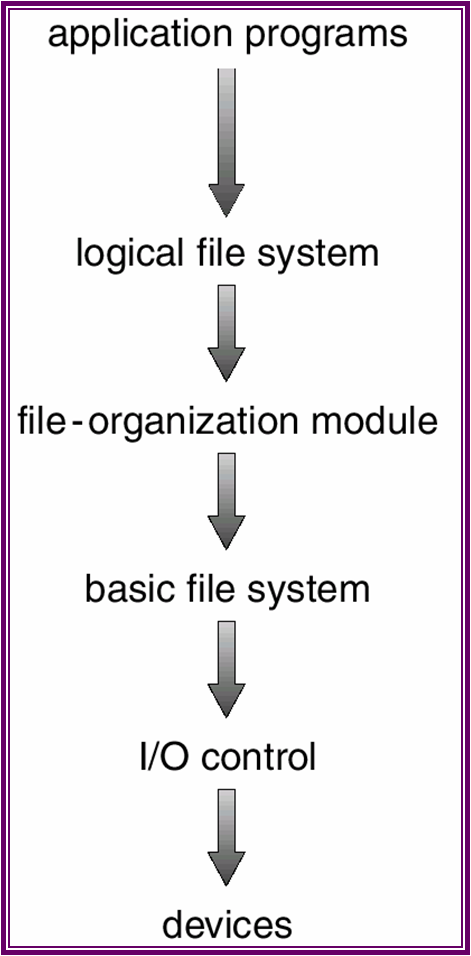
\includegraphics[scale=.4]{v6f12-1}
    \end{center}
  \end{frame}
\fi
  
  %% PAGE
  \begin{frame}
    \frametitle{A typical file control block} \pause
    \begin{center}
      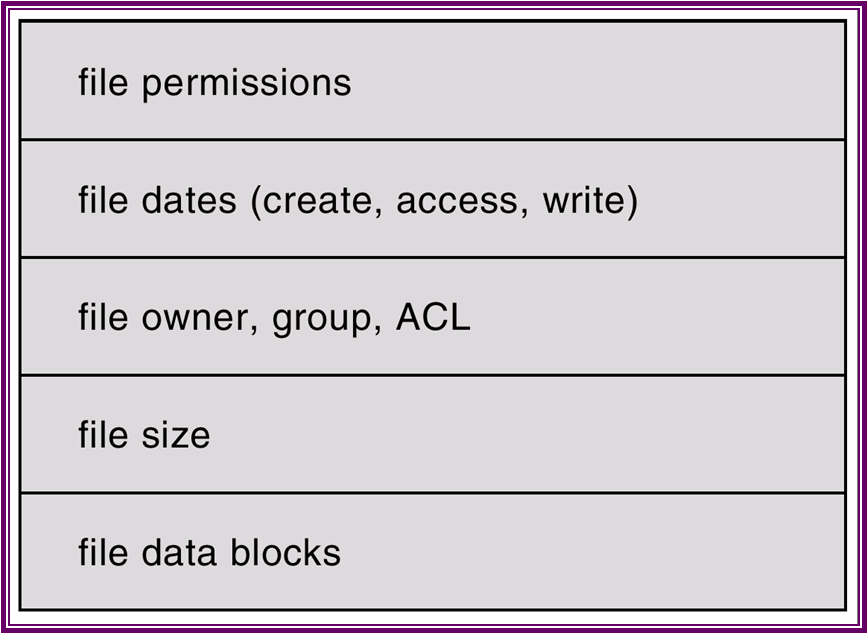
\includegraphics[scale=.5]{v6f12-2}
    \end{center}
  \end{frame}
  
  %% PAGE
  \begin{frame}
    \frametitle{On-disk file system structure (1/2)} \pause
    \begin{center}
      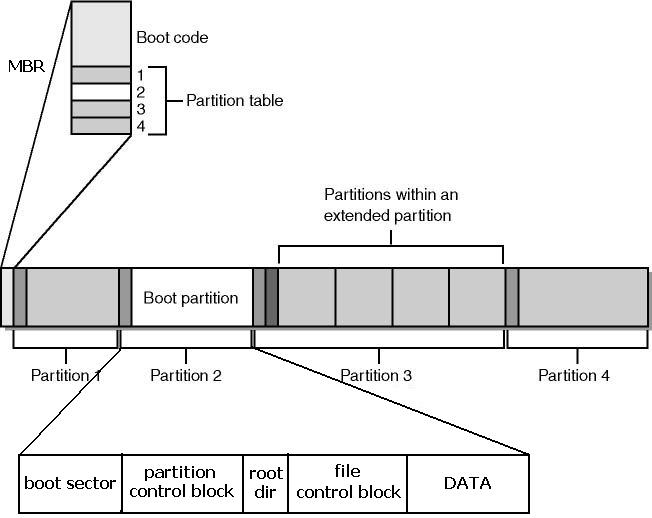
\includegraphics[scale=.5]{disklayout}
    \end{center}
  \end{frame}
  
  %% PAGE
  \begin{frame}
    \frametitle{On-disk file system structure (2/2)} \pause
    \begin{itemize}\parskip=0pt
    \item The ``boot sector'' contains codes used to load the operating system kernel when booting; \pause
      \begin{itemize}\parskip=0pt
      \item It's also known as the ``boot block'' and loaded by the code within the MBR. \pause
      \end{itemize}
    \item The ``partition control block'' contains the partition details such as number of blocks in the partition, size of blocks, free-block count and free-block pointers, and free FCB count and free FCB pointers. \pause
      \begin{itemize}\parskip=0pt
      \item It's also known as ``superblock'' in UNIX or ``Master File Table'' in Windows NT.
      \end{itemize}
    \end{itemize}
  \end{frame}
  
  %% PAGE
  \begin{frame}
    \frametitle{In-memory file system structure} \pause
    \begin{itemize}\parskip=0pt
    \item An in-memory partition table containing information about each mounted partition \pause
    \item An in-memory directory structure that holds the directory information of recently accessed directories \pause
    \item The \emph{system-wide open-file table} contains a copy of FCB of each open file, as well as other information \pause
    \item The \emph{per-process open-file table} contains a pointer to the appropriate entry in the system-wide open-file table, as well as other information
    \end{itemize}
  \end{frame}
  
  %% PAGE
  \begin{frame}
    \frametitle{Open-file table} \pause
    \begin{center}
      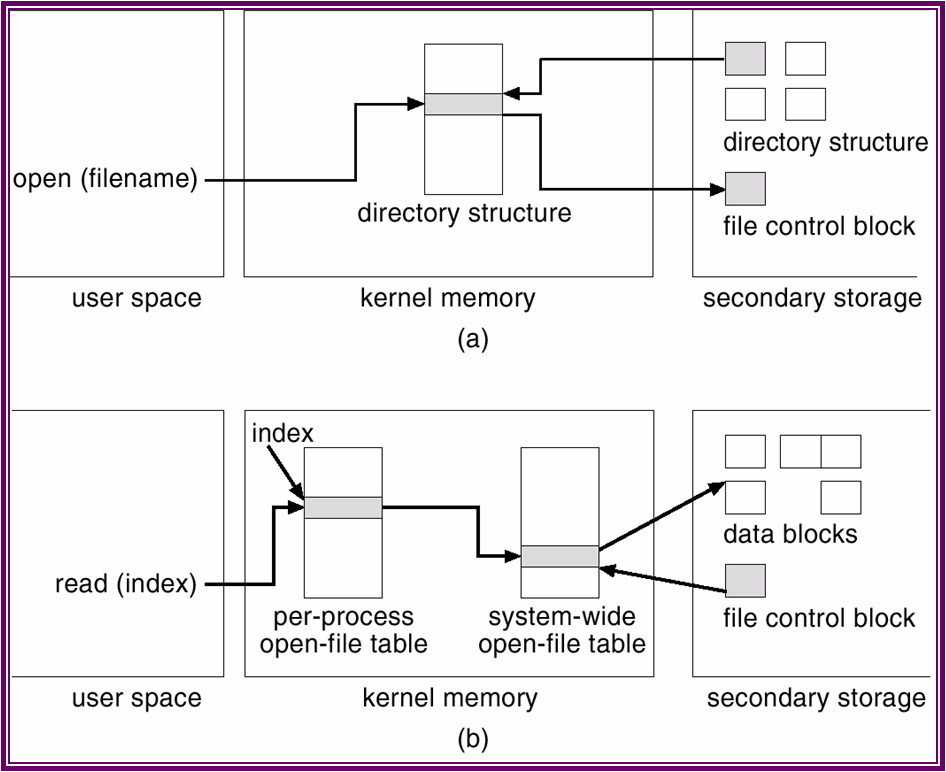
\includegraphics[scale=0.4]{v6f12-3} \pause
    \end{center}
    \begin{itemize}\parskip=0pt
    \item The ``index'' in the above figure is known as \emph{file descriptor} in UNIX or \emph{file handle} in Windows NT. \pause
      \begin{itemize}\parskip=0pt
      \item It's the value returned by the system call ``open'' in UNIX or ``CreateFile'' in Windows NT
      \end{itemize}
    \end{itemize}
  \end{frame}
  
  %% PAGE
  \begin{frame}
    \frametitle{Questions}
    \begin{itemize}
    \item Any questions?
    \end{itemize}
    \begin{center}
      
\includegraphics[scale=.5]{question}
    \end{center}
  \end{frame}
  
  \subsection{File system implementation}

  %% PAGE
  \begin{frame}
    \frametitle{Virtual File System (VFS)} \pause
    \begin{itemize}\parskip=0pt
    \item Why VFS? \pause
      \begin{itemize}\parskip=0pt
      \item The types of file system are as many as the flavors of ice cream. \pause
      \item How does an operating system allow multiple types of file systems to be integrated into one directory structure? \pause
      \item How can users seamlessly move between file system types as they navigate a directory? \pause
      \end{itemize}
    \item Most operating systems use object-oriented techniques to simplify, organize and modularize the implementation \pause
      \begin{itemize}\parskip=0pt
      \item A common file system interface is separated from the file system implementations \pause
      \item The file system interface contains the system calls such as ``open'', ``close'', ``read'', ``write'' and ``seek'', etc.
      \end{itemize}
    \end{itemize}
  \end{frame}
  
  %% PAGE
  \begin{frame}
    \frametitle{Schematic view of a VFS (1/2)} \pause
    \begin{center}
      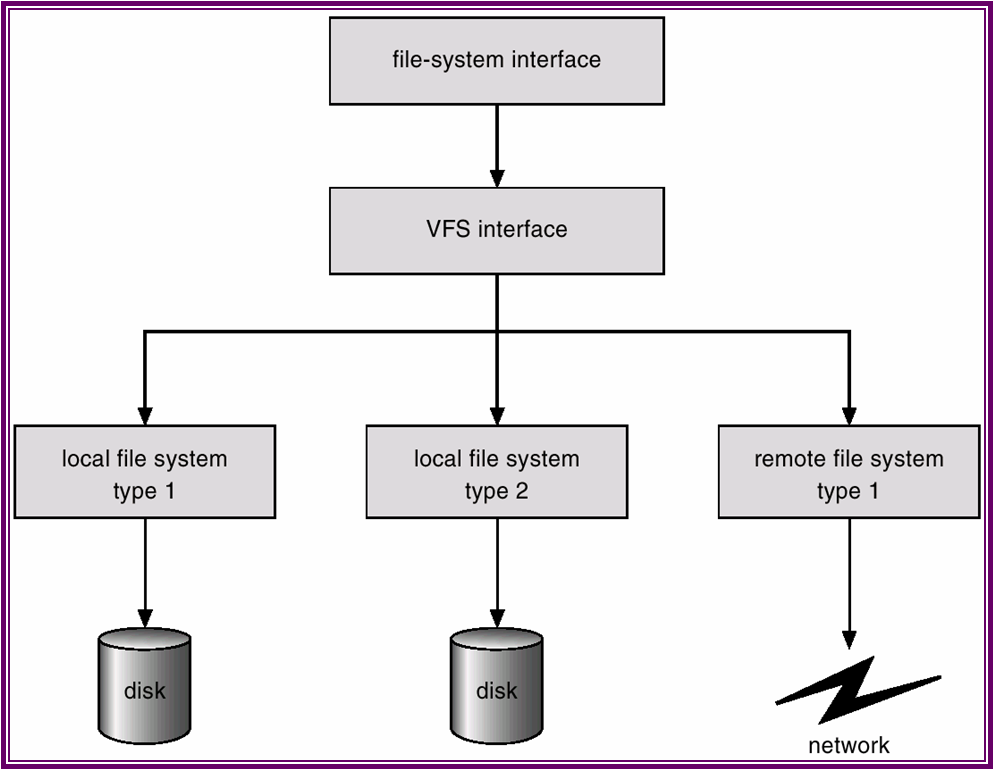
\includegraphics[scale=.5]{v6f12-4}
    \end{center}
  \end{frame}
  
  %% PAGE
  \begin{frame}
    \frametitle{Schematic view of a VFS (2/2)} \pause
    \begin{itemize}\parskip=0pt
    \item The ``VFS interface'' serves two important functions: \pause
      \begin{itemize}\parskip=0pt
      \item It separates file-system-generic operations from their implementation by defining a clean VFS interface \pause
      \item The VFS is based on a file-representation structure, called a \emph{vnode}, that contains a numerical designator for a network-wide unique file
      \end{itemize}
    \end{itemize}
  \end{frame}
  
  %% PAGE
  \begin{frame}
    \frametitle{Questions}
    \begin{itemize}
    \item Any questions?
    \end{itemize}
    \begin{center}
      
\includegraphics[scale=.5]{question}
    \end{center}
  \end{frame}

  \subsection{Directory implementation}
  
  %% PAGE
  \begin{frame}
    \frametitle{Directory implementation} \pause
    \begin{itemize}\parskip=0pt
    \item Some operating systems, including UNIX, treat a directory exactly as a file \pause
      \begin{itemize}\parskip=0pt
      \item It holds two pieces of information for each file or sub-directory within it: \emph{file/subdir name} and \emph{a pointer to the FCB of the file/subdir} (they are usually organized into a C ``struct dirent'') \pause
      \end{itemize}
    \item A directory may contain a lot of files or subdirectories, how to organize these ``dirent''? \pause
      \begin{enumerate}\parskip=0pt
      \item Linear list \pause
        \begin{itemize}\parskip=0pt
        \item Simple to program \pause
        \item Time-consuming to search \pause
        \end{itemize}
      \item Hash table \pause
        \begin{itemize}\parskip=0pt
        \item Decrease search time \pause
        \item Difficult to grow \pause
        \end{itemize}
      \end{enumerate}
    \item Most operating systems use the ``Linear list'' to organize a directory.
    \end{itemize}
  \end{frame}
  
  %% PAGE
  \begin{frame}
    \frametitle{Questions}
    \begin{itemize}
    \item Any questions?
    \end{itemize}
    \begin{center}
      
\includegraphics[scale=.5]{question}
    \end{center}
  \end{frame}

  \subsection{Allocation methods}
  
  %% PAGE
  \begin{frame}
    \frametitle{Allocation methods} \pause
    \begin{itemize}\parskip=0pt
    \item How to allocate data blocks to files so that disk space is utilized effectively and files can be accessed quickly? \pause
    \item Three major methods of allocating \pause
      \begin{enumerate}\parskip=0pt
      \item Contiguous allocation \pause
      \item Linked allocation \pause
      \item Indexed allocation
      \end{enumerate}
    \end{itemize}
  \end{frame}
  
  %% PAGE
  \begin{frame}
    \frametitle{Contiguous Allocation} \pause
    \begin{itemize}\parskip=0pt
    \item Each file occupies a set of contiguous blocks on the disk \pause
    \item Pros and cons \pause
      \begin{itemize}\parskip=0pt
      \item Simple: only starting block and length (number of blocks) are saved in FCB \pause
      \item Support random access and cache friendly \pause
      \item Suffer from the \emph{external fragmentation} \pause

        \begin{itemize}\parskip=0pt
        \item The problem of \emph{dynamic storage allocation} \pause
        \end{itemize}

      \item Difficult to grow a file
      \end{itemize}
    \end{itemize}
  \end{frame}
  
  %% PAGE
  \begin{frame}
    \frametitle{An example} \pause
    \begin{center}
      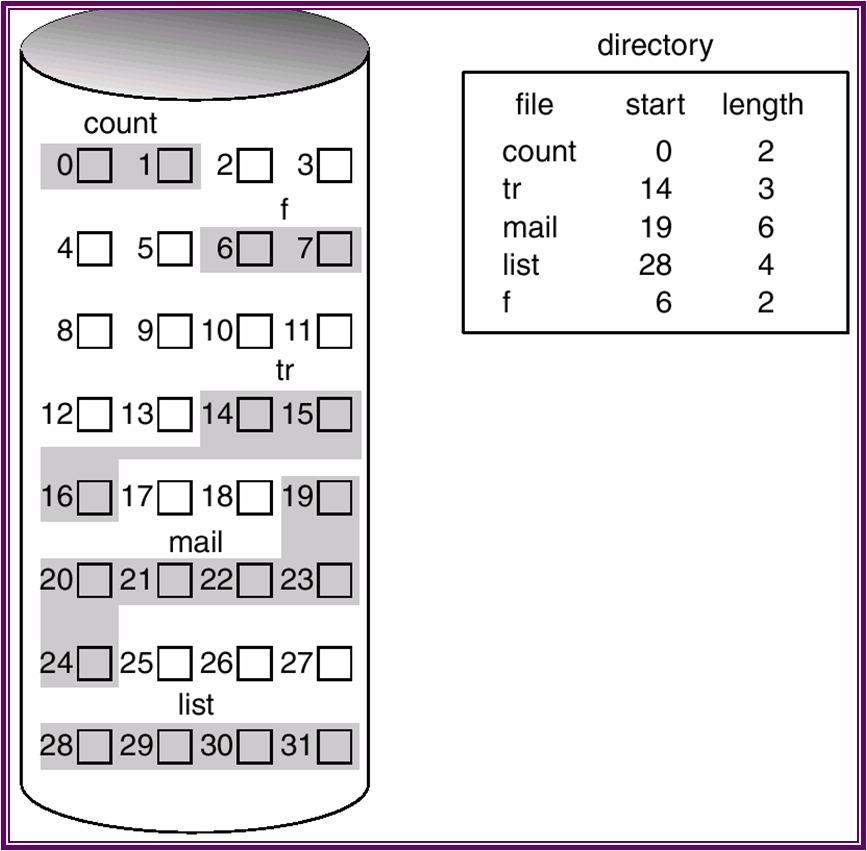
\includegraphics[scale=.5]{v6f12-5}
    \end{center}
  \end{frame}
  
  %% PAGE
  \begin{frame}
    \frametitle{Linked Allocation} \pause
    \begin{itemize}\parskip=0pt
    \item Each file is a linked list of data blocks \pause
      \begin{itemize}\parskip=0pt
      \item The FCB contains a pointer to the first and last blocks of the file \pause
      \item Each block contains a pointer to the next block \pause
        \begin{itemize}\parskip=0pt
        \item These pointers are not visible to the user \pause
        \item Thus, if data block is 512 bytes and a block address (the pointer) requires 4 bytes, then the user sees blocks of 508 bytes \pause
        \end{itemize}
      \end{itemize}
    \item Pros and cons \pause
      \begin{itemize}\parskip=0pt
      \item Simple: need only starting address \pause
      \item No waste of space \pause
      \item Extra space required for the pointer \pause
      \item No random access \pause
      \item Bad reliability because of scattered pointers \pause
      \end{itemize}
    \item The overhead of the pointers can be decreased by collecting several blocks into one larger block called a \emph{cluster}
    \end{itemize}
  \end{frame}
  
  %% PAGE
  \begin{frame}
    \frametitle{File Allocation Table (FAT)} \pause
    \begin{itemize}\parskip=0pt
    \item To solve the problem of simple linked allocation, a section of disk at the beginning of each partition is set aside to contain a table which contains all the pointers of the file system. \pause
      \begin{itemize}\parskip=0pt
      \item This table is called \emph{File Allocation Table (FAT)} \pause
      \end{itemize}
    \item An example \pause
    \end{itemize}
    \begin{center}
      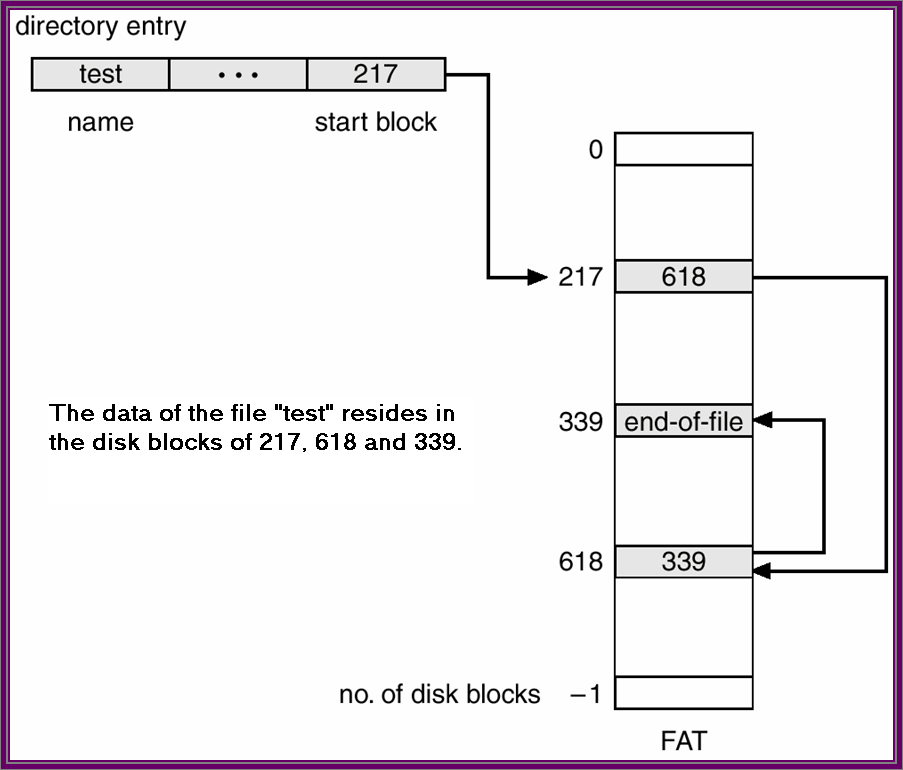
\includegraphics[scale=0.18]{v6f12-7}
    \end{center}
  \end{frame}
  
  %% PAGE
  \begin{frame}
    \frametitle{FAT file system} \pause
    \begin{itemize}\parskip=0pt
    \item The above linked allocation with FAT is used by the MS-DOS and OS/2 operating systems. \pause
      \begin{itemize}\parskip=0pt
      \item It's well known as the FAT file system \pause
      \end{itemize}
    \end{itemize}
    \begin{center}
      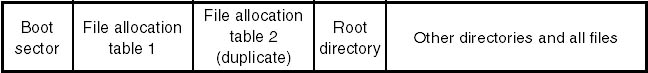
\includegraphics[scale=0.4]{fat} \pause
    \end{center}
    \begin{itemize}\parskip=0pt
    \item An example (FAT16) \pause
    \end{itemize}
    \begin{center}
      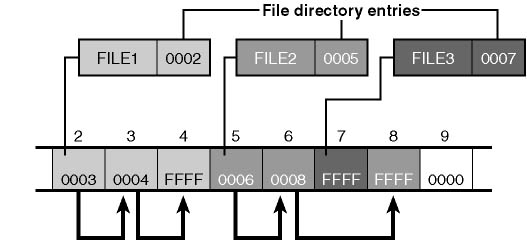
\includegraphics[scale=0.4]{fateg}
    \end{center}
  \end{frame}
  
  %% PAGE
  \begin{frame}
    \frametitle{Questions}
    \begin{itemize}
    \item Any questions?
    \end{itemize}
    \begin{center}
      
\includegraphics[scale=.5]{question}
    \end{center}
  \end{frame}
  
  %% PAGE
  \begin{frame}
    \frametitle{Indexed Allocation} \pause
    \begin{itemize}\parskip=0pt
    \item Bring all pointers to data blocks of a file together into one location: \emph{index block} \pause
      \begin{itemize}\parskip=0pt
      \item The index block holds an array of data-block addresses \pause
      \end{itemize}
    \item Pros and cons \pause
      \begin{itemize}\parskip=0pt
      \item Need index table \pause
      \item Random access \pause
      \item Dynamic access without external fragmentation, but have overhead of index block.
      \end{itemize}
    \end{itemize}
  \end{frame}
  
  %% PAGE
  \begin{frame}
    \frametitle{An example of indexed allocation} \pause
    \begin{center}
      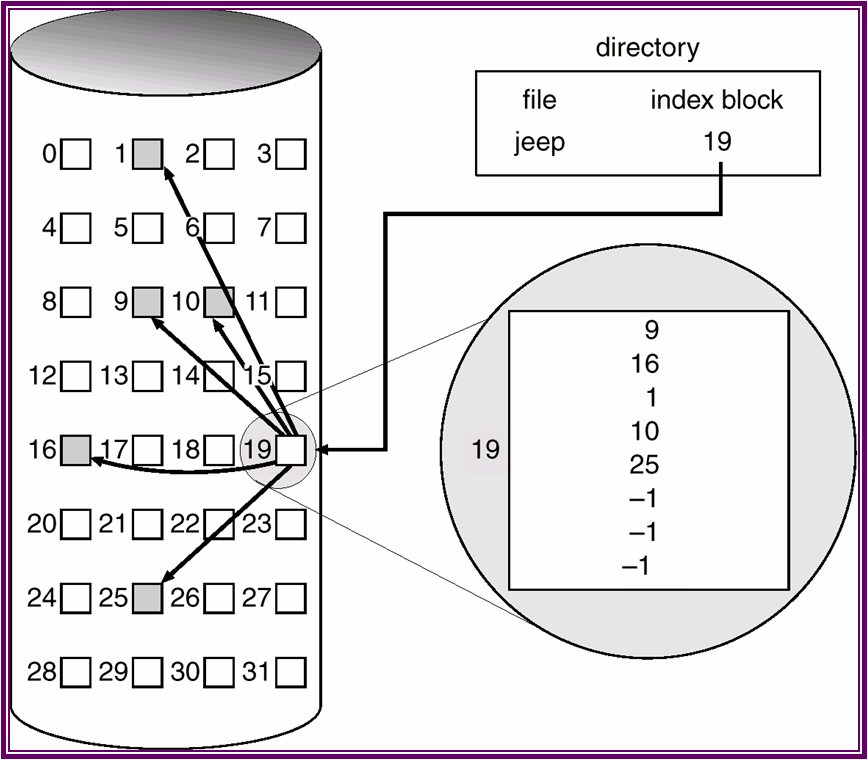
\includegraphics[scale=.5]{v6f12-8}
    \end{center}
  \end{frame}
  
  %% PAGE
  \begin{frame}
    \frametitle{The index block} \pause
    \begin{itemize}
    \item How large should the index block be? \pause
    \item Three schemes: \pause
      \begin{enumerate}\parskip=0pt
      \item Linked scheme \pause
      \item Multi-level index \pause
      \item Combined scheme of above two \pause
        \begin{itemize}\parskip=0pt
        \item This is scheme used by most UNIX file systems
        \end{itemize}
      \end{enumerate}
    \end{itemize}
  \end{frame}
  
  %% PAGE
  \begin{frame}
    \frametitle{An example} \pause
    \begin{itemize}\parskip=0pt
    \item The FCB of the UNIX file system, i.e., the \emph{inode} \pause
    \end{itemize}
    \begin{center}
      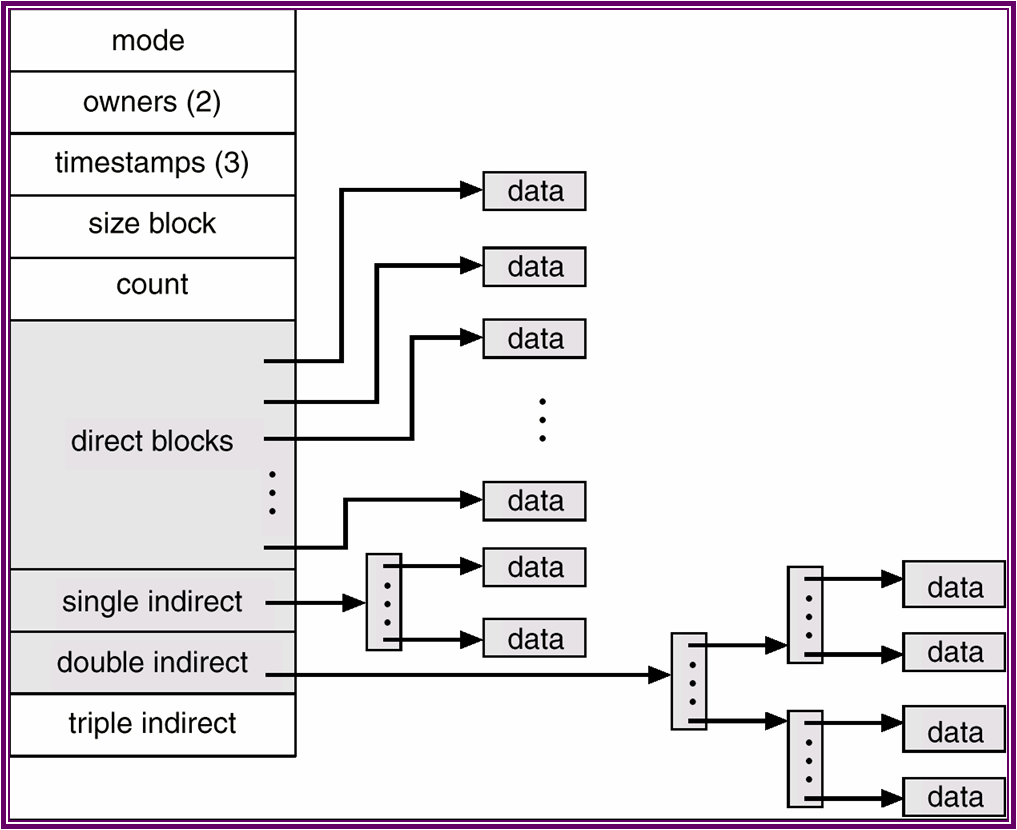
\includegraphics[scale=.5]{v6f12-9}
    \end{center}
  \end{frame}
  
  %% PAGE
  \begin{frame}
    \frametitle{Questions}
    \begin{itemize}
    \item Any questions?
    \end{itemize}
    \begin{center}
      
\includegraphics[scale=.5]{question}
    \end{center}
  \end{frame}
  
  \subsection{Free-space management}

  %% PAGE
  \begin{frame}
    \frametitle{Free space management} \pause
    \begin{itemize}\parskip=0pt
    \item Since disk space is limited, we need to reuse the space from deleted files for new files, if possible. \pause
      \begin{itemize}\parskip=0pt
      \item Hence, the free space within a file system must be recorded for allocation to new files \pause
      \end{itemize}
    \item Usually, one of the two methods is used \pause
      \begin{enumerate}\parskip=0pt
      \item Bit vector \pause
      \item Linked list
      \end{enumerate}
    \end{itemize}
  \end{frame}
  
  %% PAGE
  \begin{frame}
    \frametitle{Bit vector} \pause
    \begin{itemize}\parskip=0pt
    \item It's also known as \emph{bit map} \pause
    \item Each block is represented by 1 bit \pause
      \begin{itemize}\parskip=0pt
      \item If the block is free, the bit is 1 \pause
      \item If the block is allocated, the bit is 0 \pause
      \end{itemize}
    \item Pros and cons \pause
      \begin{itemize}\parskip=0pt
      \item Simple and efficient in finding the first free block, or \emph{n} consecutive free blocks on the disk \pause
        \begin{itemize}\parskip=0pt
        \item Because many CPUs supply bit-manipulation instructions \pause
        \end{itemize}
      \item Easy to get contiguous blocks
      \item Bit vector must be kept in the memory to be efficient and in the disk to be persistent \pause
        \begin{itemize}\parskip=0pt
        \item Assume block size = $2^{12}$ bytes and disk size = $2^{30}$ bytes (1 gigabyte), then \emph{n}=$2^{30}/2^{12}=2^{18}$ (32K bytes)
        \end{itemize}
      \end{itemize}
    \end{itemize}
    % \begin{center}\parskip=0pt
    %   \includegraphics[scale=.5]{bitvector} \pause
    % \end{center}
  \end{frame}
  
  %% PAGE
  \begin{frame}
    \frametitle{Questions}
    \begin{itemize}
    \item Any questions?
    \end{itemize}
    \begin{center}
      
\includegraphics[scale=.5]{question}
    \end{center}
  \end{frame}
  
  %% PAGE
  \begin{frame}
    \frametitle{Linked list} \pause
    \begin{itemize}\parskip=0pt
    \item Link together all the free disk blocks and keep a pointer to the first free block in a special location on the disk and cache it in memory for efficiency \pause
    \item Pros and cons \pause
      \begin{itemize}\parskip=0pt
      \item The link pointer (except the link head) is saved within the free blocks, low space overhead \pause
      \item It's not efficient to traverse the list to get free blocks \pause
        \begin{itemize}\parskip=0pt
        \item Cache several addresses of the free blocks at beginning
        \end{itemize}
      \end{itemize}
    \end{itemize}
  \end{frame}
  
  %% PAGE
  \begin{frame}
    \frametitle{An example} \pause
    \begin{center}\parskip=0pt
      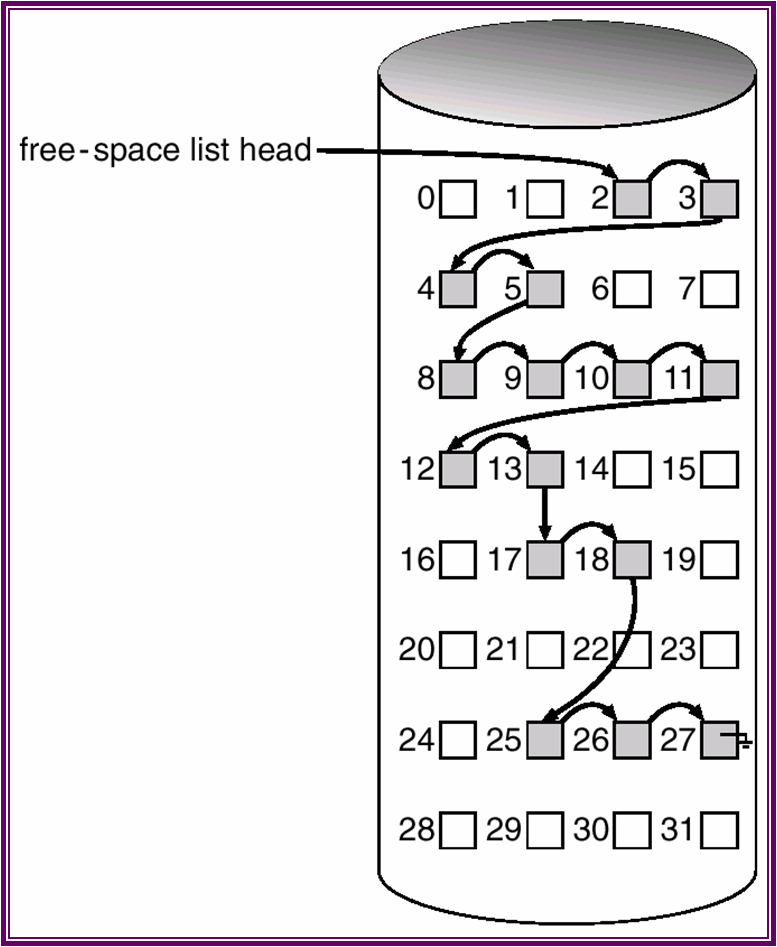
\includegraphics[scale=.4]{v6f12-10}
    \end{center}
  \end{frame}
  
  %% PAGE
  \begin{frame}
    \frametitle{Questions}
    \begin{itemize}
    \item Any questions?
    \end{itemize}
    \begin{center}
      
\includegraphics[scale=.5]{question}
    \end{center}
  \end{frame}

  \subsection{Efficiency and performance}
  
  %% PAGE
  \begin{frame}
    \frametitle{Performance} \pause
    \begin{itemize}\parskip=0pt
    \item If every disk access requires the disk operations, such as rotation, seek, access and transfer, \pause
      \begin{itemize}\parskip=0pt
      \item system performance must be bad \pause
      \item disk should be busy and its lifetime be short \pause
      \end{itemize}
    \item We need caches at following three levels: \pause
      \begin{enumerate}\parskip=0pt
      \item In the disk controller: \emph{track cache} \pause
      \item In the operating system: \emph{disk cache} \pause
        \begin{itemize}\parskip=0pt
        \item Best known as the \emph{buffer cache} \pause
        \end{itemize}
      \item In the user program: \emph{RAM disk}
      \end{enumerate}
    \end{itemize}
  \end{frame}
  
  %% PAGE
  \begin{frame}
    \frametitle{Buffer cache} \pause
    \begin{center}
      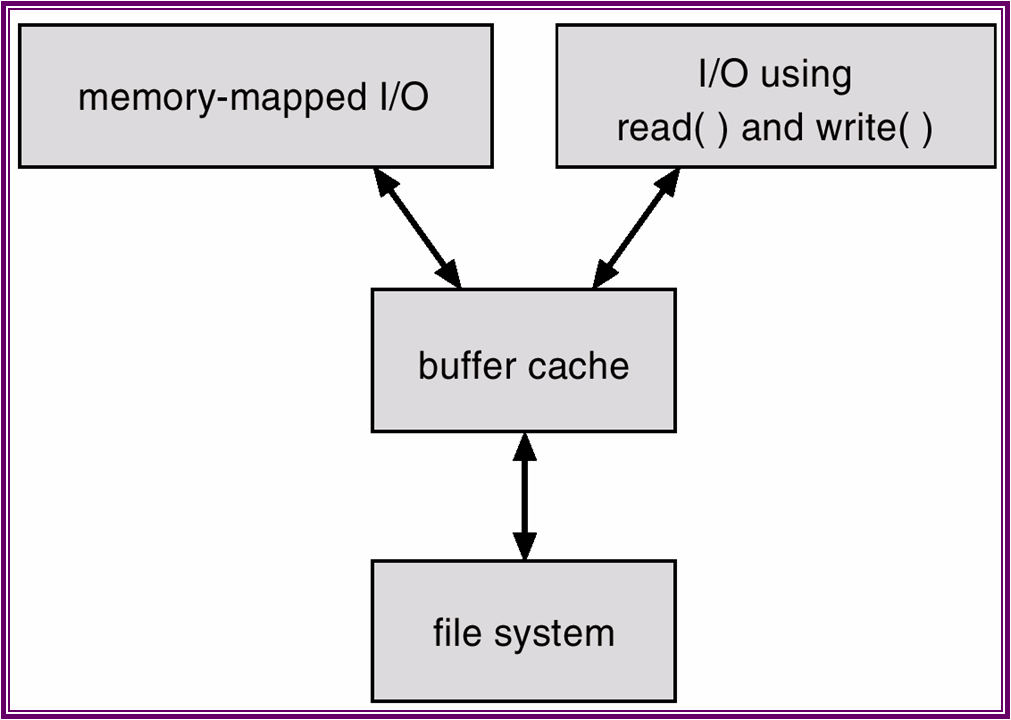
\includegraphics[scale=.4]{v6f12-12} \pause
    \end{center}
    \begin{itemize}\parskip=0pt
    \item It's typically a separate portion of the main memory \pause
    \item It controls performance by selecting replacement algorithms \pause
      \begin{itemize}\parskip=0pt
      \item \emph{read-ahead}: sequential pre-fetch \pause
      \item \emph{free-behind}: remove a block as soon as its access is completed
      \end{itemize}
    \end{itemize}
  \end{frame}
  
  %% PAGE
  \begin{frame}
    \frametitle{RAM disk} \pause
    \begin{itemize}\parskip=0pt
    \item A portion of memory is set aside and treated as a \emph{virtual disk} \pause
      \begin{itemize}\parskip=0pt
      \item The RAM disk device driver accepts all the standard disk operations, but performs those operations on the memory, instead of on a disk \pause
      \end{itemize}
    \item Unfortunately, RAM disks are only useful for temporary storage, since its contents will be lost between reboots
    \end{itemize}
  \end{frame}
  
  %% PAGE
  \begin{frame}
    \frametitle{Questions}
    \begin{itemize}
    \item Any questions?
    \end{itemize}
    \begin{center}
      
\includegraphics[scale=.5]{question}
    \end{center}
  \end{frame}
  
  %% PAGE
\end{CJK*}
\end{document}
